\section{Inverse filter}
The first and most obvious type of deconvolution is using an inverse filter. We have a blurred image $g$, we found an estimation of the psf ($h_e$) in the previous section %TODO ça sera tjs des sections ?
. So we are theoretically ready to find the original image. We had
\begin{equation}
 g =  h*f,
\end{equation}
in frequency domain
\begin{equation}
G = HF. 
\end{equation}

Using $H_e$, the estimated psf in frequency domain, we can get $F_e$ an so $f_e$ by 
\begin{equation}
F_{e} = H_{e}^{-1} G
\end{equation} 

However it's clear that if we add some noise this model doesn't work anymore. Indeed as shown on figure \ref{fig:psfFFT}, $H_e$ has some value near zero. So when we divide $G$ by this, the noise is strongly amplified by the value near zero. This problem explains the results obtained on figure XXX. %TODO  

\begin{figure}
\centering
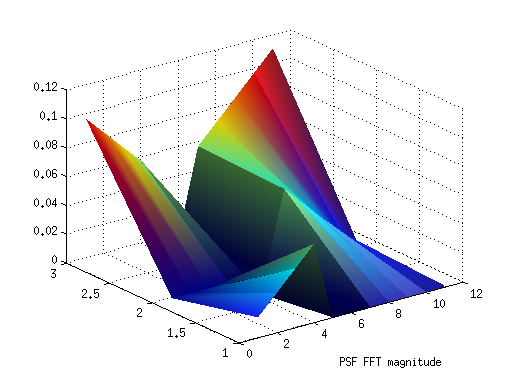
\includegraphics[scale=0.5]{../Images/psfFFT.png}
\caption{FFT of the psf}
\label{fig:psfFFT}
\end{figure}



\section{Lucy Deconvolution}



\section{Wiener Deconvolution}
 Another deconvolution is the wiener one. 




\section{Regularisation}
%TODO
The last deconvolution method is the deconvolution using regularized filter. 
Instead of a simple inverse 
\begin{equation}
\sum_{m,n} \left[ (g(m,n) - h(m,n)*f(m,n))^2 + \alpha (l(m,n)*f(m,n))^2 \right]
\end{equation}

\begin{equation}
\sum_{k,l} \{ [G(k,l) - H(k,l)F(k,l)]^2 + \alpha [L(k,l)F(k,l)]^2\}
\end{equation}


\begin{equation}
\hat{F}(k,l) = \frac{H(k,l)}{|H(k,l)|^2 + \alpha |L(k,l)|^2} G(k,l)
\end{equation}